\section{The theory}\label{sec:crit-theory}

The parts of the theory are correct. The centre is not: the paper contains two economies, a stationary one in which the main theorem is stated and a life-cycle one in which everything is quantified, and the first is neither a special case nor a limit of the second. Most of what follows comes from that.

\subsection{The central step: from the frontier value to output}\label{sec:crit-lemma4}

\subsubsection{What goes wrong}
Lemma~4 says that output per researcher equals $aF$. Its premise is that every option a free researcher takes is worth $F$. Lemma~2 gives the count of who is producing: a share $e^{-\rho T}$ of a stationary topic's members. Put the two together. Output per member is $a\,v\,e^{-\rho T}$. Entry makes $v\,e^{-(\rho+\xi)T}=F$. Hence
\[
\text{output per member}=a\,F\,e^{\xi T}\quad\text{and not}\quad aF .
\]
At the calibration ($T=0.74$ years, $\xi=0.04$) the factor is 1.030. Counting explorers, output per researcher is 2.6\% above $aF$ without founders and 1.2\% above with them.

\subsubsection{Why}
The two exponents answer different questions. A newcomer discounts her payoff by $e^{-(\rho+\xi)T}$, because she may leave, \emph{or the topic may die}, before she has caught up. The cross-section count $e^{-\rho T}$ is right only if the members who were there at a topic's birth did not have to catch up. Those members never paid the entry cost. They hold $\xi/(\rho+\xi)=29\%$ of producer-years, and for them ``every option is worth $F$'' is false: they earn more.

So the stationary benchmark mixes two conventions about how a topic is born:

\begin{center}\small
\begin{tabularx}{\textwidth}{@{}P{2.1in}LL@{}}
\toprule
Convention & Used in & Implication \\
\midrule
(a) A topic is born without a stock; its first members are insiders at once & Lemma 2's member count; Remark 6; Proposition 9 & Early cohorts earn rents; output exceeds $aF$ \\
(b) Every member pays the entry cost $T(P)$ & Lemma 4; Theorem 3; the planner's objective & Output equals $aF$ exactly, but young topics are not at the common density \\
\bottomrule
\end{tabularx}
\end{center}

The paper's sentence ``a newborn topic reaches the common density at once'' cannot be made consistent with either: if its first members pay no catch-up they earn more than $F$; if they do, the topic cannot have that flow for its first $T$ years.

\subsubsection{What it does to the numbers}

\begin{figure}[h]
\centering
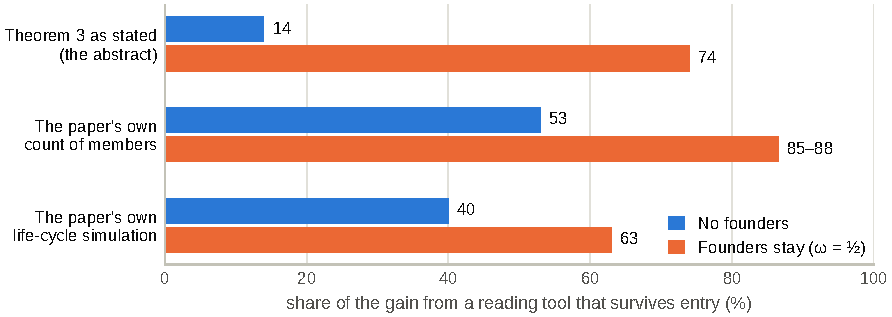
\includegraphics[width=\textwidth]{passthrough.pdf}
\caption{Share of the gain from a 30\% reading tool that survives entry, under three ways of counting. The first is what the abstract reports. The second uses the paper's own count of producing members (Lemma~2) and was obtained by re-solving the equilibrium and measuring output from that count. The third is from the paper's own Table~9.}
\label{fig:passthrough}
\end{figure}

\begin{center}\small
\begin{tabularx}{\textwidth}{@{}Lrrr@{}}
\toprule
 & As stated & Own member count & Own life cycle \\
\midrule
Reading tool, no founders & 14\% & 53\% & 40\% \\
Reading tool, founders ($\omega=\tfrac12$) & 74\% & 85--88\% & 63\% \\
Reading tool, no founders, no depletion & 0\% & 45\% & 40\% \\
Catch-up tool, no founders & 16\% & 25--28\% & 11\% \\
Per hour saved, production over reading & 1.3--7.2 & 1.15--1.9 & 1.25--2.5 \\
\bottomrule
\end{tabularx}
\end{center}

About half of a reading gain survives with no founders at all. The paper's own simulation shows the same thing: with no founders and no depletion the theorem says nothing survives, and the life cycle says 40\%. The paper prints both numbers side by side and leads with the first.

On the life cycle, output per researcher-year is 3.2\% above $F$ without founders. By phase it is $0.99F$ in growing topics (many members still reading), $1.10F$ in consolidating topics (everyone there entered during growth) and $1.04F$ in mature ones (where survivors of the growth phase write 29\% of the papers). All of the excess is the rent of cohorts that entered before entry was costly.

\begin{notebox}
The code never tests Lemma~4. \texttt{equilibrium()} in \texttt{code/ftmodel/equilibrium.py} sets output per researcher to $aF$ by construction, and the test of the incidence formula compares the formula with that. Another test asserts that output per member-year in a mature topic is $F e^{\xi T}$. The two tests pass together because they never meet.
\end{notebox}

\subsubsection{The repair, and why it is an improvement}
The response of the frontier value is correctly characterised by Theorem~3. Only the step from $F$ to output fails, and the fix is one more term:
\[
\dd\ln\frac{Y}{N}=\dd\ln a+\dd\ln F+\frac{\xi}{\rho+\xi}\Bigl(\eps_\Gamma\,\dd\ln P^*-h_\Gamma\Bigr),
\]
where $h_\Gamma$ is the tool's direct effect on the entry factor. For a learning tool the new term adds $\frac{\xi}{\rho+\xi}\,\eps_\Gamma(1-\thF)/\Psi$ to the surviving share: 0.50 without founders or depletion and $0.74+0.13=0.87$ with founders. Exact re-solves give 0.45 and 0.88.

\begin{ideabox}[The economics of the missing term]
Entry \emph{capitalises} a gain that reaches entrants into a higher barrier. A tool that raises the newcomer's payoff by $h$ draws people in until the reading needed to join has grown enough to offset it. The marginal entrant ends up no better off. Insiders do: their payoff rises by $(\eps_\Gamma/|\eps_w|)\,h$, about $1.7h$ at the calibration. A tool's gain therefore stays with whoever is \emph{inframarginal}: the people who open topics, the cohorts that entered before entry was costly, and a scarce frontier. This is a clearer claim than ``output equals the frontier'', and Part~III builds on it.
\end{ideabox}

Three further points belong here.

\emph{The stationary benchmark is not a limit of the life-cycle model.} If topics grow infinitely fast the stock vanishes and they are flooded to just below the speed limit, then thin for about eighteen years. If they grow infinitely slowly they stall. No diffusion rate reproduces the benchmark.

\emph{The planner's gain depends on the convention.} With one exponent the planner's density is 4.3 and the gain 1.25\%; with the other, 5.2 and 0.37\%. Both are smaller than the 3.0\% accounting wedge between the two conventions. The direction (topics are too crowded) is the same under both.

\emph{The paper's Table~9 compares columns that differ in two assumptions.} The ``formula'' column has depletion and values founders at maturity; the ``life cycle'' column has no depletion and puts founders on the simulated path.

\subsection{The founders' channel}\label{sec:crit-founders}

The novelty of version~3 is that founders carry tools to the frontier. Four findings limit it.

\begin{enumerate}
\item \textbf{Founders live through the growth phase.} A founder is present for $1/(\rho+\xi)=7.1$ years. The median topic needs 6.5 years to reach its mature density. So a founder's payoff on the life cycle is 1.82, against 1.95 at maturity and 1.76 at the frontier. On the life cycle the frontier receives 42\% of a reading gain and 1\% of a catch-up gain, against 74\% and 41\% in the stationary formula.
\item \textbf{``Founders stay'' is imposed, not chosen.} In the simulation 36\% of newborn topics attract no follower. Their founders earn less than the frontier value and would do better exploring again.
\item \textbf{Nothing identifies the founders' share.} No calibration moment depends on it. The founding rate is set to 0.14 ``so that half of them found one''. The symbol $\omega$ is the share of an explorer's time spent as a founder, not a probability; the probability of founding is 0.58.
\item \textbf{Varying it changes the economy.} In the life-cycle rows of the paper's table, moving $\omega$ from 0.25 to 0.75 moves the share of researchers who are exploring from 37\% to 6\%. The rows are not a change in founders' incumbency with everything else equal.
\end{enumerate}

\begin{critbox}[The headline range restates two inputs]
With founders, 74\% is the founders' share itself (55 points, from the assumed $\omega=\tfrac12$) plus 18. Without founders, 14\% is $\EE\times D=0.15\times1.11$, evaluated for a 30\% shock. Over $\omega$ from 0 to 0.75 and $\EE$ from 0 to 0.27 the surviving share runs from 0 to 93\%, and the per-hour ratio from 1.06 to 32. The lower end of ``1.3 to 7.2'' is set by an assumption. The upper end is set by the choice of $\EE$, and the paper says that the model's density is the close-radius one, where the estimate is 0.035 with a standard error of 0.118: at that value the ratio is 33, and the ``floor that the data measure'' is statistically zero.
\end{critbox}

\subsection{The ranking of tools is assumed}\label{sec:crit-ranking}

``Production tools survive almost fully; reading tools survive mainly through founders; catch-up tools least'' reads as a result. It is two assumptions.

\textbf{What explorers do.} An explorer ``produces $e$ per unit of production speed''. So the frontier value scales one for one with $a$, and $e$ does not depend on reading speed, learning, search or catch-up. With no founders and no depletion the theorem returns 100\% for production and 0\% for reading by construction; the test suite asserts this as ``full dissipation''. The level of $e$ is a calibrated residual: 1.6--1.8, when a lone researcher in an empty topic earns 1. Exploring is worth 98.8\% of what the best-organised topic pays. All long-run incidence falls on an activity the paper does not model.

\textbf{No fertility depletion.} Appendix~B.1 lets later topics be less fertile, at elasticity $\eta_f$, and shows that density data cannot identify it. Output per researcher then falls with the number of open topics. A reading tool \emph{lowers} the number of topics (by 8 log points; a catch-up tool by 27), so it gains; a production tool raises it and loses.

\begin{center}\small
\begin{tabularx}{0.8\textwidth}{@{}Lrrrrr@{}}
\toprule
Fertility depletion $\eta_f$ & 0 & 0.04 & 0.06 & 0.10 & 0.30 \\
\midrule
Reading tool: share that survives & 13\% & 58\% & 81\% & 126\% & 350\% \\
Production tool: share that survives & 99\% & 96\% & 94\% & 91\% & 74\% \\
\bottomrule
\end{tabularx}
\par\smallskip
\parbox{0.8\textwidth}{\footnotesize Re-solved with the calibrated curves, no founders. Two independent computations put the crossing at $\eta_f\approx0.055$--$0.07$.}
\end{center}

The paper's own growth section says that the measured decline in research productivity ``must come from falling fertility of new topics'' or from selection on ability. If fertility depletion is large enough to matter there, production tools do not ``survive almost fully'', and concentration of science is good, not bad. The caveat appears in Proposition~10 and is absent from Corollary~2 and from the abstract.

\textbf{One technology split in two.} Reading speed is $b=100$ papers a year; catch-up speed is $b_c=38.6$. Nothing relates the two: the first is a normalisation, the second is fitted to rents. A tool that summarises a literature speeds up both, and its incidence lies between the two rows of the paper's table.

\begin{ideabox}[The honest statement]
In the long run a tool is worth the time it saves in the activity of opening topics, plus a term for general equilibrium. Whether production tools or reading tools save more time at the frontier is an empirical question about what the people who open topics do. It can be measured: compare the reference lists and the output of papers that open a new cluster with those of papers that follow.
\end{ideabox}

\subsection{Novelty and positioning}\label{sec:crit-novelty}

In structure the incidence theorem is a known result. Lemma~4 is utility pinned at the outside option, as in the spatial equilibrium of Roback (1982), the migration model of Harris and Todaro (1970), and open-access rent dissipation (Gordon 1954). The formula of Theorem~3 is the two-curve incidence formula: a shift in the newcomer's payoff is divided according to the slope of that payoff and the slope of the frontier. The insiders' premium is the Harris--Todaro queue. There is no land in the model, so local gains are dissipated by congestion and by queueing, not capitalised into rents on land. None of these papers is in the bibliography.

What is new is the application and two features of it: the outside option contains the inside payoff, because founders stay; and tools are classified by whether they move the outside option. A search of the literature found no paper that states the incidence result for research tools. The defensible claim is the application and its measurement, not the theorem.

The speed limit is the stability condition of a queue (delay grows without bound as arrivals approach the service rate), and as economics it is the burden of knowledge of Jones (2009) with the margin of narrowing one's field shut. The take-off and overshooting results are close to models of industry shakeouts and to recent work on research waves. The closest missing references are listed in Appendix~\ref{sec:app-lit}.

\subsection{The speed limit}\label{sec:crit-speed}

\begin{figure}[h]
\centering
\begin{tikzpicture}[x=0.128cm,y=1cm,font=\sffamily\footnotesize]
\fill[gridc] (0,0) rectangle (100,0.3);
\fill[hblue] (0,0) rectangle (53,0.3);
\foreach \x in {0,25,50,75,100} {\draw[axisc,line width=0.5pt] (\x,-0.07) -- (\x,0); \node[below,color=inktwo] at (\x,-0.08) {\x\%};}
\draw[ink,line width=0.6pt] (17,0.3) -- (17,0.72) node[above,align=center,color=ink,inner sep=1.5pt] {typical mature\\topic: 17\%};
\draw[ink,line width=0.6pt] (33,0.3) -- (33,1.62) node[above,align=center,color=ink,inner sep=1.5pt] {most fertile\\mature topic: 33\%};
\draw[ink,line width=0.6pt] (53,0.3) -- (53,0.72) node[above,align=center,color=ink,inner sep=1.5pt] {highest any topic\\reaches: 53\%};
\draw[stcritdark,line width=1pt] (100,-0.04) -- (100,0.72) node[above,align=center,color=stcritdark,inner sep=1.5pt] {the speed\\limit};
\node[color=inktwo] at (76.5,0.15) {no researcher-year here};
\node[below,color=inktwo] at (50,-0.55) {a topic's flow of papers as a share of what a newcomer can read};
\end{tikzpicture}
\caption{Where the calibrated economy sits relative to the speed limit. Closing the densest mature topic requires production to triple.}
\label{fig:limit}
\end{figure}

Theorem~2 is correct as stated. Six findings say that it should not carry the title.

\begin{enumerate}
\item \textbf{It never operates.} In the simulated cross-section the ratio of a topic's flow to the limit has a median of 0.22, a 99th percentile of 0.39 and a maximum of 0.53. Only 4.6\% of researcher-years are above one third. Closing the densest mature topic needs production speed to rise by a factor of 3.05.
\item \textbf{``17\% of the limit'' is an identity.} In a mature topic $\Pm/b_c=1-\exp(-\text{premium}/\nu)$, and $\nu=(\rho+\xi)/\delta=0.56$ is fixed outside the calibration. With the same premium, a literature that loses relevance twice as fast ($\delta=0.5$) gives 31\%, and four times as fast gives 52\%. The number is the measured spread of returns passed through an assumed ratio of two rates.
\item \textbf{The limit exists because of a double standard.} A newcomer must read the \emph{whole} backlog, at 38.6 papers a year, before she may write anything. An incumbent counts as up to date while reading 7 papers a year at the mature density, 13 at the limit (a third of the flow), and never more than 19. If admission required only what incumbents actually read, no density would be closed.
\item \textbf{Part (iii) holds for myopic entry only.} With forward-looking entry a very fast topic stops above the limit. A figure caption in the paper says the opposite.
\item \textbf{The fit does not need it.} A linear catch-up cost with no limit fits the targets exactly as well (losses of 13.6 and 13.8 after the same search).
\item \textbf{There is no evidence.} The only citation is to a study of attention staying with canonical papers, which is a different mechanism. A referee will ask why the fastest-growing literature of the day has the most entrants.
\end{enumerate}

What survives is the exact catch-up formula, which is better than the linear one, and the convexity of the cost, which matters for how far fast topics overshoot. The limit itself is a remark.

\subsection{Life cycles, take-off and policy}\label{sec:crit-dynamics}

\textbf{The law of motion omits the friction it is about.} In the life-cycle model joiners add to a topic's flow the day they arrive. But a joiner writes only after she has caught up, 0.8 years at the stopping date. People who joined in the last months before entry stops are still reading, and when they start to write the flow keeps rising: by 16\% for the median topic, which carries it past the peak although its growth rate is below the overshooting threshold, and to more than double for a topic growing at 100\% a year, which carries it above the speed limit. The thresholds of Proposition~9 and the statement that entry stops below the limit are properties of a model without a catch-up delay.

\textbf{Two steps of the proof are numerical.} That a stalled topic is abandoned, and that the overshooting threshold equals the stated maximum with the exact stock, are ``verified numerically for the calibrated parameters''. Both have short proofs, which the review wrote out; random searches over parameters found no counterexample.

\textbf{Take-off is a knife-edge that no topic reaches.} The valley in which a slow topic stalls exists only for a birth flow between 1.76 and 2.68 papers a year; the paper assumes 2. In the calibrated population the slowest topic grows at 8.8\% a year, and the take-off threshold is at most 7\% for any topic that can mature. No topic stalls for slow growth. The 36--40\% of newborn topics that fail do so because they are not fertile enough at birth, a margin the paper does not discuss. With forward-looking entry the threshold falls from 2.2\% to 1.0\% a year.

\textbf{The diffusion rate carries the block and is not modelled.} How fast a topic grows rations entry and so generates every rent in the quantification. It is an exogenous random draw, and its distribution is the least well identified part of the calibration.

\textbf{The policy knife-edges are artefacts.}

\begin{center}\small
\begin{tabularx}{0.86\textwidth}{@{}Lrrrrr@{}}
\toprule
Assumed flow of a newborn topic & 1.5 & 1.8 & 2.0 & 2.5 & 3.0 \\
\midrule
Newborn margin $\ln[v(P_0)/F]$ & $-1.7\%$ & $+0.2\%$ & $+1.3\%$ & $+3.4\%$ & $+5.0\%$ \\
Largest share of learning from the stock at which topics are born & 0 & 0.02 & 0.11 & 0.27 & 0.38 \\
Stationary subsidy as a multiple of the margin & --- & --- & 0.97 & 0.37 & 0.25 \\
\bottomrule
\end{tabularx}
\end{center}

``A flat subsidy would bring the economy to the edge of the regime in which new topics attract no followers'' and ``if more than 11\% of learning drew on the stock, no new topic would ever find a follower'' both reverse with a 10\% change in an assumed number. At the better-fitting parameters found by the review (\S\ref{sec:crit-calib}) the newborn margin is 0.1\% and 48\% of topics are stillborn. What survives is the ranking: a tax that rises with a topic's stock beats a flat subsidy by a factor of 2 to 5.6, with gains of 0.13--0.72\% of output.

\subsection{A topic has two members}\label{sec:crit-size}

With the stated normalisation ($a=4$, $b=100$) a mature topic has 1.75 producers and 1.9 members. The planner's best size is 1.15 producers. A newborn topic is half a writer. One more producer raises a topic's flow by 57\% and lowers the newcomer's payoff by 5.4\%, four times the planner's whole gain. More than half of what a member ``learns from'' is her own output.

The density results do not depend on this: with $a=0.4$ a topic has 19 members and every density is unchanged. What does not survive is the language of persons: a first follower, a founder as one insider among many, entry ``one at a time'', diffusion at a continuous rate. The paper must choose between a theory of neighbourhood density (and drop the person-counting) and a rescaling in which a topic is a community of tens.

The same normalisation fixes how much is read. An incumbent reads 7 papers a year, about 20 hours each; a newcomer reads 39 papers a year full time, about 52 hours each. The survey behind the 7\% reading share counts a few hundred article readings a year of about half an hour each. One model ``paper'' is therefore about forty readings, and the paper should say what it is.
